\section{Critique of the Model itself}

    Through the process of formalizing the memory model, we also critiqued the model in a few aspects. 
    We here elicit mainly three of them which we consider to be due to under-specified semantics.

    \subsection{Tearing Factor and the Tear-free reads Axiom}

        The model states that all integer aligned accesses are tear-free.  
        In terms of hardware, whether a memory access is tear free depends also on the bus-size.
        But if we still want to declare an access at the ECMAScript language level tear-free, the hardware must adopt some way to ensure that the access is indeed tear-free, meaning they respect the tear-free axiom.
        Alternatively, if at the ECMAScript language level, we declare an access to tear despite the hardware having it to be tear-free, this would mean the compiler can perform certain aggressive optimizations to leverage this relaxation. 

        If we are using teared memory accesses, the set of observable behaviors becomes slightly non-trivial to justify.
        For instance, consider the program in Figure \ref{crit:tearing}, where we assume that $x$ represents an 12-byte memory which is initialized to zero. 
        Suppose that read to $x$ is tearing but the writes are tear-free.
        \begin{figure}[H]
            \centering
            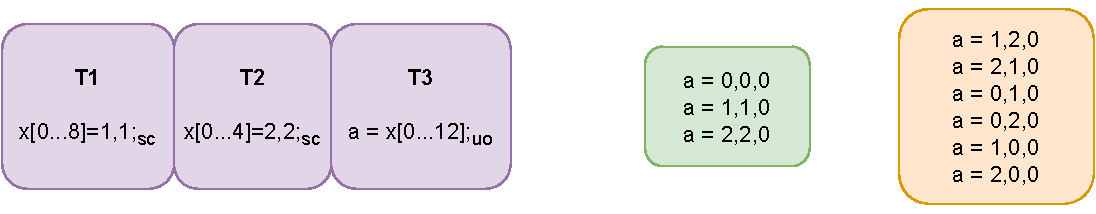
\includegraphics[scale=0.7]{6.ConclusionFutureWork/TearingExample.pdf}
            \caption{Mixed-size Tearing reads example}
            \label{crit:tearing}
        \end{figure}

        The green box represents the outcomes that we can intuitively justify.
        But the model also allows the outcomes in the orange box. 
        This is because of the read that tears, which implies that Axiom \ref{TfRe} does not constrain $stck{_{rf}}$ to be functional with respect to the read and the writes to the same 8-byte memory. 
        Whether this is left to the hardware or program transformations is uncertain.
        If so, how could one justify any of the outcomes in the orange box is yet to be understood by us. 

        The main concern is that if both the writes are tear-free as well as sequentially consistent, how is it that the read can read them as if they are teared?
        Does this mean that the tearing factor of SC events depends on the existence of reads that tear or do not tear? 
        If this is so, it would be non-trivial to reason about programs locally.
       
        Consider the same last program above but with the read also of type $sc$. 
        Yet the above two behaviors having those read values are allowed.,
        Even Axiom \ref{SeqCsAt} does not restrict such an observable behavior.

        We believe this to be a problem with the tear-free reads axiom.
        A possible direction towards resolving this is to define the notion of tear-free / tearing using read-bytes-from relation. 

    \subsection{Range of Initialize events uncertain}

        Whether the range of $init$ events is the entire shared memory buffer or is it byte-size is uncertain.
        This affects the way we can reason with our programs and their corresponding observable behaviors.

        Consider the two candidates in Figure \ref{crit:range}, each of which could represent the same program, one where the initialize event is to the whole 8-byte(right) and one where its split into two events of type $init$ writing 4 bytes each(left).
        The orange box is an observable behaviors in question.
        \begin{figure}[H]
            \centering
            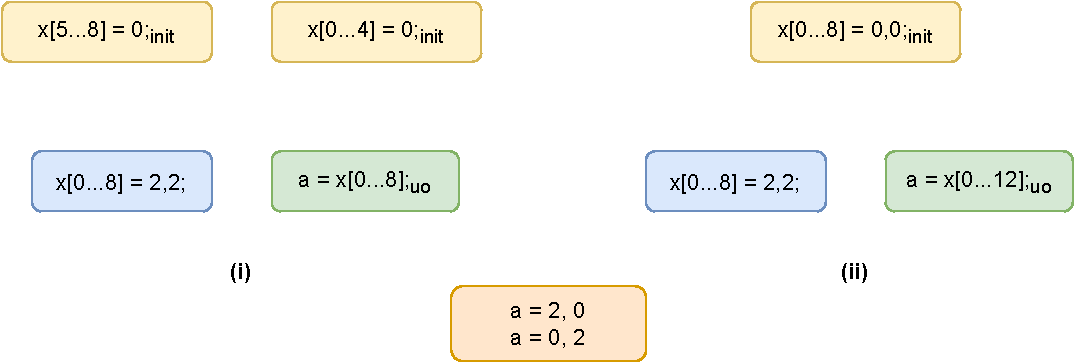
\includegraphics[scale=0.7]{6.ConclusionFutureWork/InitExample.pdf}
            \caption{Mixed-size Init events example}
            \label{crit:range}
        \end{figure}

        For the first candidate, the outcomes in question are possible.
        But for the second program, the outcomes are not possible due to Axiom \ref{TfRe}.
        Which one must correspond to the original program is unclear and is not specified by the semantics of the model.

    \subsection{Mixed-size events do not respect Coherence irrespective of access mode}

        Events that are unordered need not respect Coherence, unless constrained by happens-before relation.
        These accesses, mixed with sequentially consistent ones, give non-trivial behaviors.

        For instance, consider the program in Figure \ref{crit:coherence} with the orange box having the observable behavior in question.
        \begin{figure}[H]
            \centering
            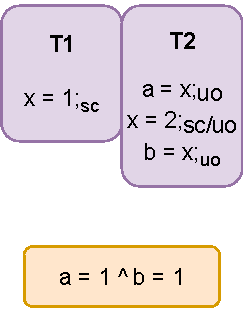
\includegraphics[scale=0.7]{6.ConclusionFutureWork/CoherenceNormal.pdf}
            \caption{Coherence violation Example.}
            \label{crit:coherence}
        \end{figure}

        The above program can have the observable behavior under question.
        But this would imply that the value of write to $x$ as $2$, though local to the subsequent read, vanishes. 
        The keen reader will note that such a behavior cannot even be explained by reordering or elimination of events.
        Note also that this outcome is possible even if the write $x=2$ has an access mode of $sc$. 

        Suppose we do have standard coherence respected. 
        In this case too, sequentially consistent accesses which are mixed size give non-trivial behaviors.
        Consider another example in Figure \ref{crit:coherence_mixed} with a few mixed size accesses, where the writes are of type $sc$.
        \begin{figure}[H]
            \centering
            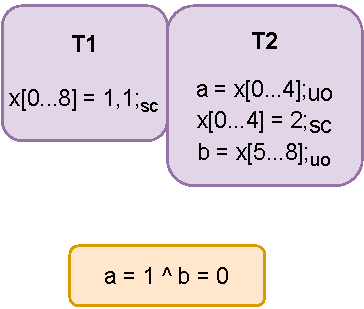
\includegraphics[scale=0.7]{6.ConclusionFutureWork/CoherenceMixed.pdf}
            \caption{Mixed-size events example where coherence is assumed to be held.}
            \label{crit:coherence_mixed}
        \end{figure}

        Here the value of read $a=x[0...4]$, despite being $1$ does not restrict the outcome of the read $b=x[5...8]$ to be $0$. 
        Again, we do not know how to justify this outcome using either reordering or elimination. 
